\documentclass[letterpaper]{article}
\usepackage{aaai}
\usepackage{times}
\usepackage{helvet}
\usepackage{courier}
\usepackage{graphicx}
\usepackage{float}
\usepackage{amsmath}
\usepackage{amssymb}
\usepackage{url}
\usepackage{booktabs}
\usepackage{xcolor}
\usepackage{tikz}
\usetikzlibrary{arrows.meta, positioning}
\frenchspacing
\setlength{\pdfpagewidth}{8.5in}
\setlength{\pdfpageheight}{11in}
\pdfinfo{
/Title (Event- and Weather-Aware Spatio-Temporal Graph Networks for Traffic Shockwave Forecasting)
/Author (Yilang Mei, Raouf Tadros, Uwe Koenig)
/Keywords (traffic forecasting, spatio-temporal graph neural networks, scheduled events, weather, PEMS-BAY)
}
\setcounter{secnumdepth}{2}

% Green placeholder marker: everything wrapped in \tbd{} is unfinished.
\definecolor{tbdgreen}{RGB}{0,130,0}
\newcommand{\tbd}[1]{\textcolor{tbdgreen}{#1}}

\makeatother

\nocopyright

\title{Event- and Weather-Aware Spatio-Temporal Graph Networks\\for Traffic Shockwave Forecasting}
\author{Yilang Mei \and Raouf Tadros \and Uwe K\"onig\\
Technical University of Munich\\
\{yilang.mei, raouf.tadros, uwe.koenig\} @tum.de
}

\begin{document}
\maketitle

\begin{abstract}
\begin{quote}
Short-term traffic forecasts feed operational decisions such as signal control, detour guidance, and transit dispatch. Their value is highest during unusual periods, for example heavy rain or the departure peak after a stadium event, yet standard benchmarks average errors over test sets dominated by routine traffic. We ask whether weather and scheduled-event information, both available before congestion forms, improve speed forecasts specifically inside such anomalous windows. On the PEMS-BAY network of 325 sensors we condition a Spatio-Temporal Graph Convolutional Network on calendar, weather, event-activity, event-magnitude, and venue-distance channels, and evaluate it inside windows defined only from schedules and weather observations, alongside a physics-level check of whether the model reproduces the upstream propagation of a shockwave. Across 144 trained configurations neither signal in our title behaves as assumed. Weather channels make the model \emph{worse} the more weather-specific the window becomes: 4.9\% worse overall, 6.6\% inside adverse weather and 8.0\% inside rain during the commute peak, with a mechanism we measured before training --- rain does not change how often breakdowns occur or how large they are, it is a uniform $-3.04$~mph capacity reduction already legible in the speed history. Event channels do lower error, but inside the egress hour a model with no event channels at all scores 1.237~mph against 1.239 for one that knows a fixture's time, venue and attendance; removing attendance changes nothing; and their gains appear in a window containing no fixtures. What helps most is the calendar, which is broadcast to every node exactly as the weather is. The distinction that survives is redundancy, not spatial structure: an exogenous channel helps when it carries what the target's own history cannot supply. Granting the model the next hour of every knowable channel, drawn for weather from an ECMWF~IFS forecast archive, does not change this: pooled over rungs and folds it is harmful at every horizon, and the one configuration it helps is the only one whose future block is both unavailable from the past and known exactly. Aggregate MAE meanwhile predicts the other error metrics (Spearman $+0.79$ against window error, $-0.65$ against onset recall) but not whether a model reproduces the $1.68\times$ upstream asymmetry that defines a shockwave ($-0.35$, $p=0.30$).
\end{quote}
\end{abstract}

\section{Introduction}

Traffic forecasts are rarely an end in themselves. Agencies use them to time signal plans, position staff, reroute busses, and warn drivers. These interventions matter most when traffic breaks from its daily pattern, for example, while rain reduces road capacity or while 17,000 hockey fans leave a downtown arena within half an hour. Such periods make up a small part of any test set. A model can therefore reduce its average error on a standard benchmark without becoming more useful in the situations where a forecast actually changes a decision.

Spatio-temporal graph neural networks are the established tool for this forecasting task. Sensors become graph nodes, road relationships become edges, and recent measurements become node-level time series. STGCN \cite{yu2018stgcn} and DCRNN \cite{li2018dcrnn} showed that this structure predicts road speeds well from historical observations alone. Later work added learned graph structure \cite{wu2019graphwavenet,bai2020agcrn} or contextual attributes such as observed incidents \cite{fan2026igstgnn}. However, An incident marker only becomes available once the disruption has started. Scheduled events and weather differ in one operationally useful way that they can be known before congestion forms.

This paper addresses two questions. First, does conditioning an STGCN on weather and scheduled-event information improve accuracy inside exogenously defined anomalous windows, rather than only in the aggregate? Second, is the error profile over distance from the venue and over congestion-onset time consistent with a shockwave that spreads outward through the road graph?

Three difficulties shape the design. Anomalous windows are rare, so aggregate metrics can bury them. Hourly weather records and irregular event schedules must be aligned to a 5-minute sensor grid without leaking future information. And an event flag broadcast identically to all 325 sensors says nothing about where the disruption originates, which is why the distance-to-venue channel carries the spatial anchor.

The intended contributions are a set of anomaly windows defined from schedules and weather rather than from the traffic signal itself, a conditioned version of an established architecture instead of a new one, and an evaluation that adds venue-distance profiles, onset timing, and an operational decision rule to the usual point-error metrics.

\section{Related Work}

\subsection{Forecasting anomalous traffic}

Most traffic benchmarks report errors averaged over all test timesteps. Lee et al.~\shortcite{lee2021empirical} compared major deep forecasting models under consistent settings and found that rankings change in intervals with abrupt speed changes. Zhang et al.~\shortcite{zhang2021hybrid} evaluated hybrid models separately under normal conditions, holidays, and adverse weather. Zhang et al.~\shortcite{zhang2023testtime} targeted extreme conditions by retrieving similar historical patterns at test time, and Kralj et al.~\shortcite{kralj2025pruning} proposed a sudden-event accuracy measure after showing that average error can stay strong while sharp slowdowns are missed. In all four studies the difficult intervals are identified from the realized traffic itself. We instead define them from event schedules and weather, which are known independently of the forecast target.

\subsection{Spatio-temporal graph forecasting}

STGCN combines Chebyshev graph convolution with gated temporal convolution \cite{yu2018stgcn}; DCRNN places diffusion convolution inside a recurrent encoder-decoder \cite{li2018dcrnn}. Graph WaveNet adds a self-adaptive adjacency matrix and dilated temporal convolutions \cite{wu2019graphwavenet}, and AGCRN learns node-specific parameters without a supplied graph \cite{bai2020agcrn}. Since our contribution is the conditioning and the evaluation protocol, we keep STGCN unchanged as the forecasting backbone rather than adding another architecture.

\subsection{External context in graph models}

AST-GCN concatenates weather and points of interest to the traffic input \cite{zhu2021astgcn}, and WeaGAN learns weather-traffic interactions through attention gates \cite{wang2023weagan}. On the event side, Li et al.~\shortcite{li2023periodic} model congestion episodes as events in a deployed system, Han et al.~\shortcite{han2024event} fuse traffic with textual event descriptions around convention centers, and GAT-Informer represents a sports event through temporal profiles around its start and end plus each node's distance from the arena \cite{song2024gatinformer}, which makes it the closest prior work. IGSTGNN models the spatial footprint and temporal decay of incidents \cite{fan2026igstgnn}. Dynamic graphs, exogenous context, and abnormal-window evaluation have thus each been studied on their own. What is missing, and what we attempt here, is a single controlled pipeline that combines structured event variables including attendance, weather, disruption-window reporting, and distance-based propagation analysis on a standard benchmark. We do not claim the first event-aware or weather-aware traffic model.

\section{Methodology}

\subsection{Problem definition}

Let the sensor network be a graph $G=(V,E,A)$ with $|V|=N=325$ sensors and a weighted adjacency matrix $A\in\mathbb{R}^{N\times N}$. At timestep $t$ the node features are $X_t\in\mathbb{R}^{N\times C}$. Given the past $L=12$ observations (60 minutes at 5-minute resolution), the task is to predict the next $H=12$ speed states:
\begin{equation}
\hat{Y}_{t+1:t+H}=f_\theta\!\left(X_{t-L+1:t},\,A\right),
\end{equation}
with $X_{t-L+1:t}\in\mathbb{R}^{L\times N\times C}$ and $\hat{Y}_{t+1:t+H}\in\mathbb{R}^{H\times N}$. Speed is the only prediction target for every configuration; the ablation varies only $C$, which ranges from $1$ (speed only) to $11$ (all context channels). Errors are reported at horizon steps 3, 6 and 12, i.e.\ 15, 30 and 60 minutes, matching the convention under which PEMS-BAY results are published \cite{wu2019graphwavenet}; the 45-minute column is included in Table~\ref{tab:full} and changes no conclusion.

\subsection{Pipeline overview}

Figure~\ref{fig:pipeline} summarizes the pipeline. Raw traffic, weather, and event records are aligned to one 5-minute index, assembled once into an eleven-channel master tensor, split into rolling chronological folds, and normalized per channel with training statistics only. Every ablation rung selects \emph{columns} of that one master tensor rather than rebuilding it, so all rungs share the same samples, the same fold boundaries and the same scaler, and their errors remain directly comparable.

\begin{figure}[t]
\centering
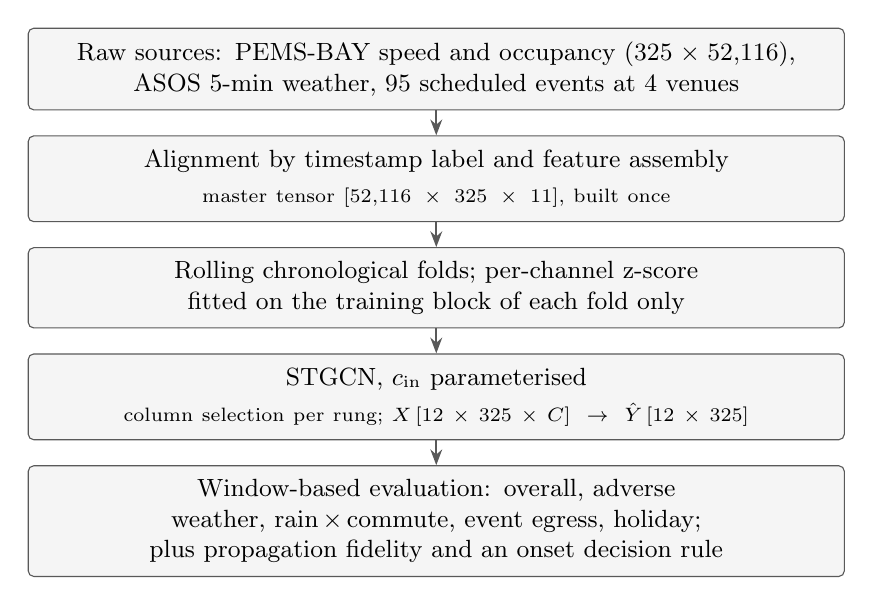
\begin{tikzpicture}[
  stage/.style={rectangle, draw=black!65, fill=black!4, rounded corners=2pt,
    text width=0.82\columnwidth, align=center, font=\small,
    inner xsep=6pt, inner ysep=5pt},
  flow/.style={-{Stealth[length=2mm]}, black!65, thick}
]
\node[stage] (a) {Raw sources: PEMS-BAY speed and occupancy ($325\times52{,}116$), ASOS 5-min weather, 95 scheduled events at 4 venues};
\node[stage, below=9pt of a] (b) {Alignment by timestamp label and feature assembly\\[2pt] {\scriptsize master tensor $[52{,}116 \times 325 \times 11]$, built once}};
\node[stage, below=9pt of b] (c) {Rolling chronological folds; per-channel z-score fitted on the training block of each fold only};
\node[stage, below=9pt of c] (d) {STGCN, $c_{\text{in}}$ parameterised\\[2pt] {\scriptsize column selection per rung; $X\,[12\times325\times C] \rightarrow \hat{Y}\,[12\times325]$}};
\node[stage, below=9pt of d] (e) {Window-based evaluation: overall, adverse weather, rain\,$\times$\,commute, event egress, holiday; plus propagation fidelity and an onset decision rule};
\draw[flow] (a) -- (b);
\draw[flow] (b) -- (c);
\draw[flow] (c) -- (d);
\draw[flow] (d) -- (e);
\end{tikzpicture}
\caption{Data and evaluation pipeline. Every stage reads only information available at forecast time; the fold boundaries and the normalization statistics never see validation or test data.}
\label{fig:pipeline}
\end{figure}

\subsection{Graph construction and samples}

Sensor identifiers, the adjacency matrix and pairwise road distances come from the Augmented PEMS-BAY release \cite{augmentedpemsbay,li2018dcrnn}. A recorded driving distance $d_{ij}$ becomes a Gaussian edge weight, and weak connections are removed:
\begin{equation}
A_{ij}=
\begin{cases}
\exp\!\left[-\left(d_{ij}/\sigma_d\right)^{2}\right] & \text{if this value} \geq 0.1,\\[2pt]
0 & \text{otherwise},
\end{cases}
\end{equation}
where $\sigma_d$ is the standard deviation of the finite recorded distances.

$A$ is \emph{directed}: it encodes driving distance, and 1{,}789 of its edges have no reverse. This matters twice, in opposite directions. Chebyshev graph convolution is defined on an undirected graph and needs a symmetric Laplacian with a real spectrum, so the backbone symmetrizes with $\max(A,A^{\!\top})$ before computing the Laplacian. Passing the raw directed matrix to a symmetric eigensolver instead returns $\lambda_{\max}=1.267$ against a true largest eigenvalue of $1.001$, mis-scaling the Chebyshev basis by 27\%. The \emph{analysis} of Section~\ref{sec:propagation}, by contrast, requires travel direction and reads the original directed matrix.

The time axis is taken from the column labels of the speed file, never regenerated: local wall-clock time in the study period is missing 2017-03-12 02:00--02:55 to daylight saving, so a naive 5-minute range yields $181\times288=52{,}128$ stamps against the 52{,}116 the data actually contains, and every later timestamp would slide by one hour. All sources are joined to that axis \emph{by label}.

\subsection{Backbone}

The backbone follows Yu, Yin, and Zhu~\shortcite{yu2018stgcn}. Two spatio-temporal blocks each apply a gated temporal convolution, a graph convolution, a second gated temporal convolution, layer normalization, dropout of 0.3, and a residual connection; both temporal convolutions use kernel size $K_t=3$, and channel widths are $[c_{\text{in}},64,64]$ and $[64,64,64]$. An output convolution over the remaining time axis and a linear layer emit all 12 horizons in one pass. The speed-only model has 116{,}940 trainable parameters and the eleven-channel model 121{,}420.

The default graph operator is the Chebyshev approximation of order $K_s=3$,
\begin{equation}
\Theta *_{G} x \;=\; \sum_{k=0}^{K_s-1}\theta_k\,T_k(\tilde{L})\,x,
\qquad
\tilde{L}=\frac{2}{\lambda_{\max}}L-I_N ,
\end{equation}
with $L=I_N-D^{-1/2}\bar{A}D^{-1/2}$ the normalized Laplacian of the symmetrized adjacency $\bar A=\max(A,A^{\!\top})$ and $T_k$ the Chebyshev polynomials. The graph convolution is general in the input width, $y_j=\sum_{i=1}^{C_{\text{in}}}\Theta_{i,j}(L)\,x_i$; Yu et al.\ instantiate it only at $C_{\text{in}}=1$, and our ablation is precisely a sweep over $C_{\text{in}}$.

We deliberately depart from the reference implementation in three places, and record them because they affect comparability rather than novelty. First, the model emits all $H$ horizons from a single forward pass, where the original predicts one step and recurses at test time; ours is the convention under which the PEMS-BAY reference numbers were published \cite{wu2019graphwavenet}. Second, the block widths are $64/64/64$ rather than the paper's bottleneck $64/16/64$, matching the configuration used for our reproduction. Third, dropout and weight decay are actually active here, whereas the released code collects a weight-decay term it never adds to the loss and feeds \texttt{keep\_prob}$=1.0$ during training.

\subsection{Exogenous conditioning}

The conditioned model widens the input from one to eleven channels and changes nothing else. Table~\ref{tab:channels} lists them together with the axis each varies over, which is the property that turns out to matter most.

\begin{table}[t]
\centering
\small
\setlength{\tabcolsep}{4pt}
\begin{tabular}{@{}rlll@{}}
\toprule
\# & Channel & Group & Varies over \\
\midrule
0 & Speed (target) & speed & node $\times$ time \\
1 & Occupancy & occupancy & node $\times$ time \\
2 & Time of day & calendar & time \\
3 & Day of week & calendar & time \\
4 & Is holiday & calendar & time \\
5 & Temperature & weather & time \\
6 & Precipitation & weather & time \\
7 & Wind speed & weather & time \\
8 & Distance to venue & event\_geo & node \\
9 & Event active decay & event\_geo & node $\times$ time \\
10 & Event load & event\_att & node $\times$ time \\
\bottomrule
\end{tabular}
\caption{The eleven input channels. Calendar and weather channels are broadcast identically to all 325 nodes; the three event channels vary across nodes through a distance kernel. Channels 2--4 pass through unnormalized; the remaining eight are z-scored.}
\label{tab:channels}
\end{table}

\paragraph{Event channels.} Each venue $e$ contributes an exponential spatial kernel over great-circle distance $d_{n,e}$ from sensor $n$,
\begin{equation}
w_{n,e}=\exp\!\left(-\,d_{n,e}/\tau\right),\qquad \tau=4\,\text{km}.
\end{equation}
Writing $W_e$ for the active interval of fixture $e$ and $A_e$ for its expected attendance, the two temporal event channels are
\begin{align}
\text{active}_{n,t} &= \sum_{e} \mathbf{1}\!\left[t\in W_e\right]\, w_{n,e},\\
\text{load}_{n,t} &= \sum_{e} \mathbf{1}\!\left[t\in W_e\right]
   \mathbf{1}\!\left[A_e \ge A_{\min}\right]
   \frac{A_e}{A_{\text{ref}}}\, w_{n,e},
\end{align}
with $A_{\text{ref}}=20{,}000$ and $A_{\min}=15{,}000$. The two differ only in whether attendance enters, which makes the pair \texttt{4\_event\_geo} versus \texttt{5\_event\_geo\_att} a controlled test of whether crowd size carries signal beyond mere fixture presence. The threshold is measured, not conventional: below 15{,}000 attendees the egress-hour speed anomaly is $+0.35\pm0.41$~mph, i.e.\ the wrong sign, while the thresholded weight reaches $t=-9.76$.

\subsection{Congestion-weighted loss}

Aggregate $L_1$ on speed is dominated by free flow: 90.4\% of observations exceed 55~mph and carry 63.7\% of the total absolute error at an MAE of 2.18, while the $<$45~mph regime is 6\% of observations carrying 26\% of the error at an MAE of 12--14. A loss averaged over all cells therefore spends most of its gradient on predicting 65~mph as 63. As a second, deliberately minimal intervention we reweight the same $L_1$ towards low speeds,
\begin{equation}
\omega(y)=1+\max\!\left(0,\ \frac{v_0-y}{\Delta}\right),
\end{equation}
\begin{equation}
\mathcal{L}=\frac{1}{|\mathcal{M}|}\sum_{i\in\mathcal{M}}\omega(y_i)\,\bigl|\hat y_i-y_i\bigr|,
\end{equation}
with $v_0=60$~mph and $\Delta=20$~mph, so $\omega=1.0$ at free flow, $1.5$ at 50~mph and $2.5$ at 30~mph. The weighting touches the objective only: architecture, channels, splits and reported metrics are unchanged, and every reported number remains \emph{unweighted} MAE, RMSE or MAPE on de-normalized mph. This is the loss-function form of the paper's own argument: if aggregate MAE hides the intervals that matter, the training objective should not be governed by it either.

\subsection{Directed graph operator}

Chebyshev convolution cannot distinguish an upstream neighbour from a downstream one, because symmetrization discards exactly the direction in which a shockwave travels. As a third intervention we replace it with the diffusion convolution of Li et al.~\shortcite{li2018dcrnn}, a dual random walk over the \emph{directed} adjacency,
\begin{equation}
Z=\sum_{k=0}^{K}\Bigl(P_{f}^{k}\,X\,\Theta_{k,1}+P_{b}^{k}\,X\,\Theta_{k,2}\Bigr),
\end{equation}
with forward and backward transition matrices $P_f=D_o^{-1}A$ and $P_b=D_i^{-1}A^{\!\top}$ on the raw directed adjacency, kept separate so the model learns a different weight upstream and downstream. Nothing else changes: the layer computes $\sum_k S_k x W_k$ and is indifferent to what the supports $S_k$ are, so only their count moves, from $K_s$ to $1+2(K_s-1)$ --- at $K_s=3$ the supports are $[I,P_f,P_f^2,P_b,P_b^2]$, five instead of three, which adds exactly 16{,}384 parameters ($4\times64\times64$) in both the speed-only and the eleven-channel model.

\subsection{Known-future covariates}
\label{sec:future}

Every variant above forecasts from the past hour alone. That is the wrong operational assumption for nine of the eleven channels: a controller planning at 17:00 already knows it will be a Tuesday at 18:00, already holds a weather forecast, and has known the fixture's start time for months. As a fourth intervention we widen the input block from $L$ past steps of every channel to $L$ past steps plus the next $H$ steps of the \emph{knowable} ones, sampled at $L$ evenly spaced offsets over $[L,L+H-1]$ so that the tensor shape and hence the backbone are unchanged. Speed and occupancy are never duplicated --- that would be reading the target. \texttt{dist\_to\_venue} is not duplicated either: it is constant in time, so its future value is bit-identical to its present one. Eight channels remain, and a rung's future block contains only those of the eight it already carries in the past block, which makes each \texttt{\_\_future} run a controlled test against its own base rung: same fold, same seeds, same target, one extra input block of $1$--$8$ channels at a uniform $448$ parameters each, so $448$ for \texttt{4\_event\_geo} and $3{,}584$ for \texttt{6\_all}.

For weather this required a different data source. Using the observed record as its own forecast is leakage, so the future weather block is drawn from the ECMWF~IFS short-range \emph{forecast} archive --- what was predicted at the time, not what happened. Validated against the observed series it agrees on 94.9\% of hours but recalls only 61.4\% of the wet ones, and that gap is itself a result below. The loader raises rather than silently substituting observed values if the forecast file is absent.

\subsection{Rolling evaluation and window definitions}
\label{sec:protocol}

\paragraph{Why not a single chronological split.} California's wet season is January to April, so \emph{any} chronological 70/10/20 split of this period puts every rain episode in the training block. We verified this: the single-split test block contains \textbf{zero} adverse-weather episodes. A weather-conditioned model cannot differ from a traffic-only one there, whatever it has learned. We therefore use expanding-window rolling folds with a 28-day test block, a 7-day validation block and a minimum 28-day training block.

\paragraph{Fold selection.} Folds are selected by the exogenous content of their test block, which is known from schedules and weather records \emph{before} any model is trained. Folds 3--5 contain zero adverse-weather episodes and zero NHL fixtures and cannot inform either research question, so all results use folds 00--02, which between them hold all 51 rain episodes and all 19 NHL fixtures that reach any test block.

\paragraph{Windows.} All four evaluation windows are derived from a weather observation or a published schedule, never from speed or occupancy; the endogenous alternative is only available after congestion has already formed, and is the definition this work exists to contrast against.
\emph{Adverse weather} is precipitation $\ge 0.51$~mm, the 75th percentile of wet steps ($-2.22$~mph mean anomaly). \emph{Rain\,$\times$\,commute} intersects it with weekdays 07--10 and 15--19. \emph{Event egress} is the hour following the scheduled end of a fixture with $A_e\ge15{,}000$. \emph{Holiday} is the five US federal holidays in the period.

\paragraph{Episodes, not timesteps.} Neighbouring 5-minute steps and neighbouring sensors are strongly correlated, so a standard error over node-timesteps understates the true uncertainty by roughly $\sqrt{n_{\text{steps}}/n_{\text{episodes}}}$. We therefore report the number of \emph{episodes} behind every window, and never attach an error bar to a window backed by fewer than about ten.

\paragraph{A confound we do not hide.} An in-window versus out-of-window ratio is always confounded, because a window sits at a particular hour and season rather than being a random sample. Two of ours show it plainly. Event egress reads \emph{easier} than its complement, not because fixtures make traffic predictable but because egress falls at 21:30--23:00 on an empty network. Rain\,$\times$\,commute reads 1.75--2.93$\times$ its complement, which invites ``rain triples the error'', but decomposing it $2\times2$ shows time of day alone accounts for a factor of 2.55 on dry samples in all three folds, with rain adding between $-0.65$ and $+1.16$~mph on top and not even agreeing in sign. Windows are the right place to \emph{look}; they do not by themselves \emph{attribute}. Every comparison in this paper is therefore model-against-model inside one window, read down a column.

\subsection{Metrics}
\label{sec:metrics}

Point error is reported as MAE, RMSE and masked MAPE on de-normalized speed, the masked variant excluding cells below 1~mph where a percentage error is noise. Those three are standard; the two definitions below are not, and they carry the part of the evaluation this paper adds.

\paragraph{Shockwave label.} A cell is in shockwave onset when speed has fallen sharply and is now low:
\begin{equation}
s_{n,t}=\mathbf{1}\!\left[v_{n,t-3}-v_{n,t}>10\ \text{mph}\right]\cdot
        \mathbf{1}\!\left[v_{n,t}<45\ \text{mph}\right].
\end{equation}

\paragraph{Propagation fidelity.}
\label{sec:propagation}
Let $E_d=\{(i,j):A_{ij}>0,\ i\neq j\}$, so that $j$ is reachable driving from $i$ and hence \emph{downstream} of $i$. A shockwave travels the other way: $j$ breaks down first and $i$ follows. We count ordered co-occurrences in both directions at lag $\ell$ and report their ratio,
\begin{equation}
R(\ell)=\frac{\sum_{(i,j)\in E_d}\sum_t s_{j,t}\,s_{i,t+\ell}}
             {\sum_{(i,j)\in E_d}\sum_t s_{i,t}\,s_{j,t+\ell}} .
\end{equation}
$R=1$ would mean the label is picking up network-wide congestion rather than a travelling wave, so this doubles as a sanity check on the label itself. Evaluated on the \emph{observed} series it peaks at $R=1.68$ at a 15-minute lag. Evaluated on a model's own predictions it asks a question no point-error metric asks: has the model learned a travelling wave, or a smooth conditional mean that happens to have low MAE?

\paragraph{Onset recall and false alarms.} A reactive rule acts once congestion is observed: speed below 45~mph for three consecutive steps. The forecast-based policy acts as soon as the model predicts that. Onset recall is the share of observed onsets the model flags; false alarms are flags with no corresponding onset. Because false alarms and misses carry asymmetric costs, and because the two users of this forecast sit at opposite ends of that asymmetry, we sweep the miss-to-false-alarm cost ratio over $\{1,2,5,10,20,50\}$ rather than committing to one operating point.

\section{Experiment}

\subsection{Data and descriptive statistics}

The study covers 1 January to 30 June 2017 in the San Francisco Bay Area. Table~\ref{tab:data} lists the three sources.

\begin{table}[t]
\centering
\small
\begin{tabular}{@{}p{0.17\columnwidth}p{0.31\columnwidth}p{0.37\columnwidth}@{}}
\toprule
Source & Size & Variables \\
\midrule
PEMS-BAY \cite{li2018dcrnn,augmentedpemsbay} & 325 sensors, 52{,}116 5-min steps & speed, occupancy, sensor metadata, road distances \\
\addlinespace
Weather \cite{iem_asos} & 2 ASOS stations (SJC, NUQ), 5-min grid & temperature, precipitation, wind speed \\
\addlinespace
Scheduled events & 95 fixtures, 4 venues & start/end, venue, coordinates, attendance, type, provenance \\
\bottomrule
\end{tabular}
\caption{Data sources for January--June 2017.}
\label{tab:data}
\end{table}

\paragraph{Traffic.} Missing speed values are rare (521 of $52{,}116\times325$ cells) and interpolated linearly in time. The target is heavily skewed towards free flow: 90.4\% of observations exceed 55~mph, 3.6\% fall in 45--55, 2.1\% in 35--45 and 3.9\% below 35.

\paragraph{Events.} The table holds 27 NHL, 24 AHL, 9 MLS and 35 concert or other fixtures, at SAP Center (69), Shoreline Amphitheatre (12), Avaya Stadium (9) and Levi's Stadium (5); 67 meet the 15{,}000-attendee threshold. Venue coordinates were cross-checked against Nominatim and Wikidata. Provenance is carried per row: only 37 fixtures have an attendance figure verified against a published box score, and the remaining 58 carry a per-type default we assigned ourselves. That distinction is not bookkeeping. Stratifying the egress-hour effect by it, the 37 verified fixtures show a speed anomaly of $-0.63\pm0.26$~mph and a shockwave odds ratio of $5.25\times$ ($z=3.66$), whereas the default-attendance tier shows $+0.18\pm0.11$ and no effect. Filtering by an attendance threshold alone would filter our own defaults.

\paragraph{Weather.} Thirteen ASOS stations cover the region; SJC and NUQ alone place every sensor within 13.2~km, while the eight outer stations win zero sensors and two nearby ones report no night observations at all. Interpolating from two points is rank-one, which is a real limitation and the reason the weather channels carry no spatial structure. The precipitation field \texttt{p01i} is a backward one-hour accumulation forward-filled across the following twelve 5-minute steps, so it \emph{cannot be summed}; thresholds and episode counts are unaffected because they are per-step comparisons.

\paragraph{Measured effects, before any training.} Adverse weather lowers speed by $2.22$~mph on average. The egress hour of an evening NHL fixture at SAP Center lowers it by $1.69\pm0.51$~mph within 2~km. Holidays are the \emph{largest} exogenous effect and the sign is positive: Memorial Day runs $+9.50$~mph in the morning peak and $+11.27$ in the evening, because a holiday removes the commute rather than adding a crowd. Holidays are therefore reported as a separate stratum and never merged into ``adverse''.

\subsection{Preprocessing}

Weather and event records are joined to the speed file's own timestamp labels. Weekends and holidays are \emph{kept}, against Yu et al., who drop them to eliminate atypical traffic: 46 of our 95 fixtures fall on a weekend, and discarding them would discard half the phenomenon. Sliding windows of 12 input and 12 target steps are cut, the folds of Section~\ref{sec:protocol} are applied, and each channel is z-scored with statistics from that fold's training block only; the three calendar channels pass through unnormalized so that a 0/1 holiday flag is not averaged with miles per hour and millimetres. The master tensor is built once and rungs select columns from it.

\subsection{Splits}

Table~\ref{tab:folds} gives the three folds and their exogenous content. The imbalance is the point: it is why folds 3--5 are excluded and why the conventional split cannot be used at all.

\begin{table}[t]
\centering
\small
\setlength{\tabcolsep}{4pt}
\begin{tabular}{@{}lrlrrr@{}}
\toprule
Fold & Train & Test block & Rain & Events & Hol. \\
\midrule
fold00 &  6{,}048 & 01-29\,--\,02-26 & 27 &  4 & 1 \\
fold01 & 14{,}112 & 02-26\,--\,03-26 & 12 & 10 & 0 \\
fold02 & 22{,}141 & 03-26\,--\,04-23 & 12 &  8 & 0 \\
\addlinespace
\textit{fold03--05} & \textit{114{,}807} & \textit{04-23\,--\,06-30} & \textit{0} & \textit{5} & \textit{1} \\
\textit{single 70/10/20} & \textit{36{,}449} & \textit{05-25\,--\,06-30} & \textit{0} & \textit{3} & \textit{1} \\
\bottomrule
\end{tabular}
\caption{Rolling folds. ``Train'' counts samples; rain, events and holidays are \emph{episodes} in the test block. The excluded rows are shown for contrast: folds 3--5 hold 73\% of the total training compute and zero rain episodes, and the conventional chronological split holds none either.}
\label{tab:folds}
\end{table}

\subsection{Setup}

Sixteen variants are trained on three folds with three seeds each, for 144 runs: the seven ablation rungs; \texttt{0\_speed} and \texttt{6\_all} again with the congestion-weighted loss, and again with the diffusion operator; and the five rungs that carry at least one knowable channel again with known-future covariates (Section~\ref{sec:future}). Optimization uses Adam at learning rate $10^{-3}$, weight decay $10^{-4}$, batch size 64, gradient clipping at 5.0 and a StepLR schedule (step 10, factor 0.7), with early stopping on validation MAE at patience 20; runs stopped between 65 and 100 epochs. Training used one NVIDIA H200 NVL at roughly 3~s per epoch. Two trivial baselines frame the learned models: persistence repeats the last observed speed, and the historical average predicts each sensor's mean speed for each slot of the week from training data alone.

\subsection{Reproduction of the speed-only backbone}

Before adding any channel we reproduced vanilla STGCN on plain PEMS-BAY under the conventional split. Table~\ref{tab:repro} compares three seeds against the STGCN values Wu et al.~\shortcite{wu2019graphwavenet} report. We note that the PEMS-BAY reference numbers everyone quotes come from that paper, not from Yu et al.~\shortcite{yu2018stgcn}, who evaluated on BJER4 and PeMSD7 with a month-based split.

\begin{table}[t]
\centering
\small
\setlength{\tabcolsep}{4.5pt}
\begin{tabular}{@{}lcccccc@{}}
\toprule
 & \multicolumn{2}{c}{MAE (mph)} & \multicolumn{2}{c}{RMSE (mph)} & \multicolumn{2}{c}{MAPE (\%)} \\
\cmidrule(lr){2-3}\cmidrule(lr){4-5}\cmidrule(l){6-7}
Horizon & ours & ref. & ours & ref. & ours & ref. \\
\midrule
15 min & 1.44 & 1.36 & 3.06 & 2.96 & 3.03 & 2.90 \\
30 min & 1.93 & 1.81 & 4.36 & 4.27 & 4.35 & 4.17 \\
60 min & 2.58 & 2.49 & 5.83 & 5.69 & 6.25 & 5.79 \\
\bottomrule
\end{tabular}
\caption{Speed-only STGCN on PEMS-BAY under the conventional split: mean over seeds 42--44 against the reference values of Wu et al.~(2019). The gap stays within 0.1~mph MAE at every horizon. \emph{Caveat.} These runs predate a correction to the Chebyshev rescaling: \texttt{eigsh} assumes a symmetric matrix and does not check, so on the directed adjacency it returned $\lambda_{\max}=1.2670$ against a true $1.0013$ and the spectrum sat in $[-1,0.58]$. The reproduction has not been repeated since that fix, so it establishes that the loader, sample slicing and training loop are sound, but not the graph operator in its current form.}
\label{tab:repro}
\end{table}

\subsection{Main result}

Table~\ref{tab:main} is the central result. Reading down any single column is meaningful; reading across is the mistake the paper is about.

\begin{table*}[t]
\centering
\small
\setlength{\tabcolsep}{4pt}
\begin{tabular}{@{}lcccccc@{}}
\toprule
Model & $C$ & Overall MAE $\downarrow$ & Rain$\times$commute $\downarrow$ & Event egress $\downarrow$ & Propagation $\uparrow$ & Onset recall $\uparrow$ \\
\midrule
\texttt{0\_speed} (published STGCN) & 1 & 2.502 & 5.349 & 1.307 & 1.375 & 0.702 \\
\texttt{1\_traffic}                 & 2 & 2.369 & 5.147 & 1.250 & 1.452 & 0.726 \\
\texttt{2\_calendar}                & 5 & \textbf{2.279} & \textbf{4.861} & \textbf{1.237} & \textbf{1.489} & 0.750 \\
\texttt{3\_weather}                 & 5 & 2.485 & 5.559 & 1.302 & 1.454 & 0.688 \\
\texttt{4\_event\_geo}              & 4 & 2.318 & 5.070 & 1.255 & 1.348 & 0.763 \\
\texttt{5\_event\_geo\_att}         & 5 & 2.303 & 4.991 & 1.239 & 1.324 & 0.752 \\
\texttt{6\_all}                     & 11 & 2.361 & 5.283 & 1.406 & 1.389 & 0.738 \\
\addlinespace
\texttt{0\_speed} + weighted        & 1 & 2.596 & 5.774 & 1.356 & 1.306 & 0.747 \\
\texttt{6\_all} + weighted          & 11 & 2.356 & 5.275 & 1.304 & 1.376 & \textbf{0.780} \\
\texttt{0\_speed} + diffusion       & 1 & 2.503 & 5.372 & 1.304 & 1.246 & 0.701 \\
\texttt{6\_all} + diffusion         & 11 & 2.338 & 5.418 & 1.329 & 1.315 & 0.740 \\
\addlinespace
persistence                         & -- & 3.043 & 7.183 & 1.400 & --- & 0.654 \\
historical average                  & -- & 2.776 & 5.973 & 1.826 & --- & 0.770 \\
\midrule
\emph{observed truth}               & & & & & \emph{1.683} & \\
\bottomrule
\end{tabular}
\caption{The 99 contemporaneous runs: mean over 3 seeds $\times$ 3 folds at the 60-minute horizon, MAE in mph. The three rungs at $C=5$ have near-identical parameter counts (118{,}732, 118{,}284 for \texttt{4\_event\_geo}) and differ only in what their added channels contain. Rank correlation of overall MAE with rain$\times$commute MAE is $+0.79$ ($p=0.004$), with onset recall $-0.65$ ($p=0.032$), and with propagation fidelity $-0.35$ ($p=0.298$).}
\label{tab:main}
\end{table*}

\begin{table}[t]
\centering
\scriptsize
\setlength{\tabcolsep}{2.6pt}
\begin{tabular}{@{}lcccccc@{}}
\toprule
 & \multicolumn{4}{c}{Overall MAE} & \multicolumn{2}{c}{Window MAE @60} \\
\cmidrule(lr){2-5}\cmidrule(l){6-7}
Model & 15 & 30 & 45 & 60 & adv.\ wx & rain$\times$cmt \\
\midrule
\texttt{0\_speed}             & 1.392 & 1.865 & 2.214 & 2.502 & 2.743 & 5.349 \\
\texttt{1\_traffic}           & 1.371 & 1.810 & 2.116 & 2.369 & 2.576 & 5.147 \\
\texttt{2\_calendar}          & 1.370 & 1.788 & 2.062 & \textbf{2.279} & \textbf{2.508} & \textbf{4.861} \\
\texttt{3\_weather}           & 1.402 & 1.868 & 2.206 & 2.485 & 2.747 & 5.559 \\
\texttt{4\_event\_geo}        & 1.372 & 1.793 & 2.079 & 2.318 & 2.547 & 5.070 \\
\texttt{5\_event\_geo\_att}   & 1.370 & 1.789 & 2.070 & 2.303 & 2.534 & 4.991 \\
\texttt{6\_all}               & 1.395 & 1.830 & 2.124 & 2.361 & 2.716 & 5.283 \\
\addlinespace
\texttt{0\_speed}+weight.     & 1.412 & 1.906 & 2.280 & 2.596 & 2.879 & 5.774 \\
\texttt{6\_all}+weight.       & 1.402 & 1.832 & 2.118 & 2.356 & 2.671 & 5.275 \\
\texttt{0\_speed}+diff.       & 1.390 & 1.864 & 2.213 & 2.503 & 2.741 & 5.372 \\
\texttt{6\_all}+diff.         & 1.390 & 1.820 & 2.108 & 2.338 & 2.708 & 5.418 \\
\addlinespace
persistence                   & 1.568 & 2.157 & 2.628 & 3.043 & 3.306 & 7.183 \\
hist.\ average                & 2.776 & 2.776 & 2.776 & 2.776 & 3.061 & 5.973 \\
\bottomrule
\end{tabular}
\caption{Full error table, MAE in mph. The 45-minute column is included because the error a 60-minute row reports is dominated by free flow: a per-node AR(12) extrapolator is out by 17.56~mph below 35~mph at 60 minutes against 5.35~mph at 15, while its aggregate column moves only from 1.63 to 3.20. No conclusion changes between the two horizons. Episodes per fold: adverse weather 27/12/12, rain\,$\times$\,commute 10/4/2, event egress 4/10/8.}
\label{tab:full}
\end{table}

\paragraph{Neither signal in the title works the way we assumed.} Table~\ref{tab:main} is read down a column. The two exogenous groups the paper is named for both fail, in different ways, and the group we added only for completeness wins.

\paragraph{Weather channels make the model worse, and worse the more weather-specific the window.} \texttt{3\_weather} against \texttt{1\_traffic} --- the same model with three channels added --- is $+0.116$~mph overall ($4.9\%$ worse), $+0.170$ inside adverse weather ($6.6\%$) and $+0.412$ inside rain\,$\times$\,commute ($8.0\%$). It also has the worst onset recall of any trained model, $0.688$. The mechanism was measured before training. Controlling for time of day, rain changes neither how often breakdowns occur --- 91.8\% of commute-peak timesteps carry a shockwave in rain against 93.1\% dry --- nor how large they are (6.25 sensors involved against 6.46). Rain is a uniform capacity reduction of $-3.04$~mph, and a uniform slowdown is the easiest thing to read out of a speed history: the model does not need to be told it is raining, it can see that everything is 3~mph slower.

\paragraph{Event channels help, but not because they are about events.} \texttt{5\_event\_geo\_att} does beat \texttt{1\_traffic}, by $0.066$~mph overall. Three measurements say the gain is not event information. First, \emph{inside the egress hour itself}, \texttt{2\_calendar} --- which has no event channels at all --- scores $1.237$ against \texttt{5\_event\_geo\_att}'s $1.239$, a difference of $0.002$~mph. A model that has never heard of the fixture performs identically to one that knows its time, its venue and its attendance. Second, removing attendance changes nothing: \texttt{4\_event\_geo} and \texttt{5\_event\_geo\_att} differ by $0.015$~mph against a seed-and-fold spread of $\pm0.15$ to $\pm0.25$, so the raw-data contrast between activity alone ($t=-1.02$) and the thresholded attendance weight ($t=-9.76$) does not survive into a trained model. Third, the gains appear in the rain\,$\times$\,commute window, which contains no fixtures. The only mechanism consistent with all three is \texttt{dist\_to\_venue}: it is static and \emph{per-node}, and STGCN has no node embeddings, so it is the one channel that tells the model which sensor it is looking at. It is acting as a positional encoding.

\paragraph{What helps is the calendar --- and it is broadcast too.} \texttt{2\_calendar} wins on overall error, on both weather windows, on the egress window and on propagation fidelity, using three channels that are each a single number copied to all 325 nodes, structurally identical to the weather channels and at the same parameter count. So the tempting reading of the \texttt{3\_weather}/\texttt{5\_event\_geo\_att} pair --- that a channel with no spatial variation is harmful on a graph model --- is \emph{wrong}. The distinction that survives all three $C=5$ rungs is redundancy:

\begin{quote}
An exogenous channel helps when it carries something the target's own history cannot supply, and costs capacity when it does not. Rain is already visible in the speed history as a uniform slowdown. Time-of-day and day-of-week are not: sixty minutes of quiet traffic looks the same at 03:00 on a Tuesday and 11:00 on a Sunday, and only the calendar places the model in the cycle.
\end{quote}

\paragraph{What aggregate error does and does not predict.} Overall MAE ranks models almost exactly as the other \emph{error} metrics do --- Spearman $+0.79$ ($p=0.004$) against rain\,$\times$\,commute MAE and $-0.65$ ($p=0.032$) against onset recall. That is unsurprising; they are all error. It does not predict whether the model reproduces the physics: against propagation fidelity the correlation is $-0.35$ ($p=0.298$). \texttt{5\_event\_geo\_att} ranks 2nd of 11 on error and 8th on propagation; \texttt{3\_weather} ranks 8th on error and 2nd on propagation. The claim this paper defends is therefore the narrow one, and it survives: a point-error metric, however carefully stratified, does not tell you whether the model learned that jams travel backwards. The cleanest case is in the next subsection.

\paragraph{The weighted loss trades false alarms for recall at no cost in MAE.} On \texttt{6\_all}, reweighting leaves aggregate MAE unchanged ($2.361\to2.356$, against a seed and fold spread of $\pm0.25$) while raising onset recall from $0.738$ to $0.780$, at 38\% more false alarms; on \texttt{0\_speed} it costs 3.8\% of aggregate MAE for the same 4-point recall gain, at 64\% more false alarms. Whether that trade is worth taking depends on the cost ratio, and the two users of this forecast sit at opposite ends of it. A network operator pre-deploying a signal plan pays staff hours for a false alarm and hours of egress delay for a miss, a ratio of 20--50. A navigation service pays one driver a 2--5 minute detour against a measured median 1.3 and p90 5.3 minute delay for driving into the jam, a ratio of 1--3. The operator can afford false alarms but we can evaluate that decision only on 21 positives; the driver cannot afford them and we can evaluate it on 16{,}743 onsets. The decision with the most tolerance for error is the one this dataset is least able to assess.

\subsection{Letting the model see the future}

The sharpest objection to the weather result is that the model was never given a fair chance: 23.7\% of adverse-weather targets have a completely dry input window, so a contemporaneous channel cannot see the rain that is about to fall. Section~\ref{sec:future}'s variant removes that objection, and the result does not change --- but the way it fails to change identifies the condition under which a known future is worth anything at all.

\begin{table}[t]
\centering
\scriptsize
\setlength{\tabcolsep}{2.6pt}
\begin{tabular}{@{}llcccc@{}}
\toprule
Rung & Future block & \multicolumn{4}{c}{$\Delta$ MAE (future $-$ base)} \\
\cmidrule(l){3-6}
 & & 15 & 30 & 45 & 60 \\
\midrule
\texttt{4\_event\_geo}      & schedule            & \textbf{--.002} & \textbf{--.006} & \textbf{--.013} & \textbf{--.021} \\
\texttt{5\_event\_geo\_att} & sched.+attend.\ & +.003 & +.003 & +.005 & +.006 \\
\texttt{2\_calendar}        & calendar            & +.002 & +.008 & +.014 & +.011 \\
\texttt{3\_weather}         & ECMWF forecast      & +.012 & +.020 & +.030 & +.040 \\
\texttt{6\_all}             & all eight           & +.012 & +.021 & +.037 & +.051 \\
\midrule
\multicolumn{2}{@{}l}{pooled, 15 rung$\times$fold pairs} & +.005 & +.009 & +.015 & +.017 \\
\multicolumn{2}{@{}l}{\quad paired $t(14)$}              & +2.42 & +2.64 & +2.56 & +2.14 \\
\multicolumn{2}{@{}l}{\quad future better in}            & 5/15 & 4/15 & 4/15 & 4/15 \\
\bottomrule
\end{tabular}
\caption{Known-future covariates, 45 further runs. Each row is its own base rung minus itself with the next 60 minutes of its knowable channels appended; negative is better. Only \texttt{4\_event\_geo} improves, and it does so in all three folds at all four horizons. Pooled over rungs and folds the intervention is \emph{harmful} at every horizon ($p=0.030,0.020,0.023,0.051$). Differences are formed from unrounded fold means and so may differ by $0.001$ from subtracting the rounded columns of \texttt{results\_main.csv}.}
\label{tab:future}
\end{table}

\paragraph{Pooled, a known future makes the model worse.} Table~\ref{tab:future} pools the 15 rung\,$\times$\,fold pairs: the lookahead models lose $0.005$ to $0.017$~mph, worse in 11 of 15 pairs at every horizon beyond 15 minutes. Aggregate error, onset recall ($0.69$--$0.75$, the same band as the contemporaneous models) and propagation fidelity (every rung within one standard deviation of its base, \texttt{2\_calendar} $1.489\to1.458$, \texttt{6\_all} $1.389\to1.398$) are all unmoved or slightly worse. The best model at 60 minutes is still \texttt{2\_calendar} at $2.279$.

\paragraph{The one exception is the only channel that is both new and certain.} \texttt{4\_event\_geo} is the sole rung that improves, and it improves in all twelve fold\,$\times$\,horizon cells, monotonically in the horizon: $-0.002$, $-0.006$, $-0.013$, $-0.021$~mph at 15, 30, 45 and 60 minutes. Growing with lead time is the signature of genuine lookahead value, and it moves the rung from 6th to 3rd overall ($2.318\to2.297$). The three failures are each informative in a different way, and jointly they give a condition. A known-future channel pays only if it is \emph{not derivable from the present} and \emph{known exactly}. The calendar fails the first: Tuesday 18:00 is a closed-form function of Tuesday 17:00, so \texttt{time\_of\_day@future} restates a channel the model already holds, buys nothing and costs $1{,}344$ parameters --- 0 of 3 folds improve. The weather forecast fails the second: it is a real forecast, recalling 61.4\% of wet hours, and feeding it in as fact injects more error than information, with the damage growing in the horizon exactly as the event gain does but with the opposite sign ($+0.012\to+0.040$). Every rung containing it degrades. Of the eight knowable channels only the event schedule satisfies both conditions --- a fixture's start time is not recoverable from an hour of speed, and it is known months ahead with certainty. Attendance fails the first condition in a weaker form: adding \texttt{event\_load@future} to the same future block cancels the entire gain ($-0.021\to+0.006$), which is the third independent measurement in this paper saying that crowd size carries nothing beyond fixture presence.

\paragraph{The weather conclusion survives its strongest test.} Weather does not help when the model sees only the past, and it does not help when the model is handed the operational forecast of the next hour either. The limitation stated by the contemporaneous experiment is therefore closed rather than outstanding, and closed in the same direction.

\subsection{Does the model learn the wave?}

Figure~\ref{fig:prop} answers Section~\ref{sec:propagation}'s question. Observed shockwave onsets travel upstream $1.68\times$ more often than downstream at a 15-minute lag. Every Chebyshev model reproduces 79--89\% of that peak at the 60-minute horizon and none collapses to 1.0, so all are learning a travelling wave rather than a smooth conditional mean --- but none reaches the truth either, and the ranking is uncorrelated with MAE.

\begin{figure}[t]
\centering
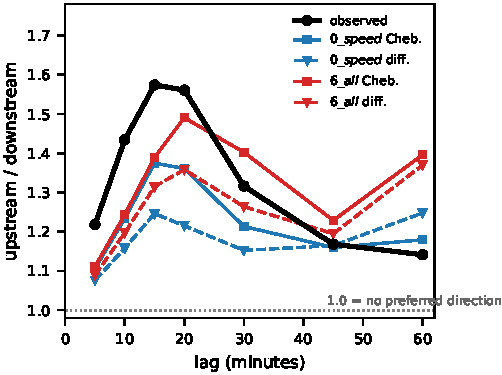
\includegraphics[width=\columnwidth]{figures/fig_propagation.pdf}
\caption{Upstream/downstream co-occurrence of shockwave onsets against lag, on the observed series and on each model's own 60-minute predictions (mean of 3 folds $\times$ 3 seeds). Every model under-reproduces the observed peak at 15 minutes. \texttt{2\_calendar} comes closest and \texttt{5\_event\_geo\_att} is among the furthest, reversing their order on point error; the directed diffusion operator, adopted to capture this very asymmetry, under-reproduces it \emph{more} than the symmetric operator it replaces.}
\label{fig:prop}
\end{figure}

\paragraph{A directed operator makes propagation worse.} The diffusion operator was adopted precisely because of that $1.68\times$ asymmetry, on the pre-registered reasoning that an operator able to tell upstream from downstream should learn a truer wave. It does the opposite. Propagation fidelity falls from $1.375$ to $1.246$ for \texttt{0\_speed} and from $1.389$ to $1.315$ for \texttt{6\_all}; paired by (fold, seed) that is $-0.129\pm0.057$ ($t=-6.73$, worse in 9 of 9 pairs) and $-0.074\pm0.100$ ($t=-2.24$, worse in 7 of 9), and it holds at the 45-minute horizon too. Aggregate MAE meanwhile moves from $2.502$ to $2.503$ and from $2.361$ to $2.338$, well inside the $\pm0.15$ to $\pm0.25$ spread across seeds and folds, so an aggregate-only report would have logged this as a small improvement while the model moved measurably further from the physics. This is the only single-variable experiment in the set --- channels, loss, data and splits are all held fixed --- and it constrains the reading of \texttt{dist\_to\_venue} above: giving the \emph{operator} the ability to distinguish upstream from downstream does not help, so what a per-node channel supplies is node identity, not a route for directional propagation.

\subsection{Negative results worth stating}

\paragraph{Compound exposure does not exist here.} Adverse precipitation during a qualifying egress hour occurs three times in six months, totalling 18 timesteps, one of them a single 5-minute step. A ``rain and event'' subset is the natural headline for a paper like this one; on this corpus it would be reporting noise, and we say so rather than constructing it.

\paragraph{Lead time cannot be reported.} The natural operational metric --- how many minutes earlier than the reactive rule the model triggers --- returns a median of \emph{zero} for all nine variants and both trivial baselines, with means below 0.35 minutes. The cause is structural rather than a property of any model: the forecast horizon is 60 minutes and the reactive rule carries its own 15-minute confirmation delay, so the resolvable range is too narrow to separate models. Onset recall and false alarms measure the same operational question and do discriminate, so we report those instead.

\paragraph{A statistic that did not survive into a model.} On the raw series the egress-hour anomaly for fixture activity alone reaches $t=-1.02$ while the thresholded attendance weight reaches $t=-9.76$, which is why the threshold was set at 15{,}000. Trained, the two rungs differ by $0.015$~mph against a $\pm0.15$--$0.25$ spread. A measured effect in the data is not the same as a usable feature, and we report both numbers rather than only the one that flatters the design.

\subsection{Limitations}

Two stations cannot express spatial weather structure, and interpolating between them is rank-one; the weather channels are consequently uniform across nodes, which Section~4 shows is the property that makes them harmful here. Venue proximity uses great-circle distance, which does not separate the carriageway that carries egress from the opposing one: 128 sensor pairs lie within 150~m on opposite carriageways, their speeds correlate at $0.115$ against $0.850$ for same-direction pairs up to 1~km apart, and switching to road-network distance strengthens the measured egress effect from $-0.41\pm0.23$ ($t=-1.75$, not significant) to $-0.89\pm0.26$ ($t=-3.37$). The event windows are small --- 4, 10 and 8 episodes per fold --- and the holiday stratum is a single case. Finally, the known-future experiment is bounded by the quality of one forecast product: the 61.4\% wet-hour recall of the ECMWF~IFS archive is what makes future weather harmful here, and a better forecast --- or a model given the forecast \emph{together with} its uncertainty rather than as a point value --- could in principle reverse that specific row without touching the condition the experiment establishes. We also test lookahead only at $H=12$; the event gain grows monotonically to the edge of that horizon, so where it saturates is unmeasured.

\section{Conclusion}

We framed traffic shockwave forecasting as an evaluation problem and then found that neither exogenous signal in our title works the way the framing assumed. Across 144 trained configurations on PEMS-BAY, weather channels make the model worse the more weather-specific the window becomes --- 4.9\% worse overall, 8.0\% inside rain during the commute peak --- because rain does not trigger breakdowns but uniformly reduces capacity by $3.04$~mph, which the speed history already shows. Event channels do lower error, yet inside the egress hour a model with no event channels matches one that knows a fixture's time, venue and attendance to within $0.002$~mph, removing attendance changes nothing, and their gains fall in a window containing no fixtures; the mechanism that fits is \texttt{dist\_to\_venue} supplying node identity to a backbone that has no node embeddings. What helps most is the calendar, broadcast to every node exactly as the weather is, which rules out the tempting conclusion that spatial variation is what matters and leaves a sharper one: an exogenous channel earns its place when it carries what the target's own history cannot supply, and costs capacity otherwise. On the evaluation side the defensible claim is narrower than we expected and it holds --- aggregate MAE ranks models as the other error metrics do (Spearman $+0.79$ and $-0.65$) but is uncorrelated with whether the model reproduces the $1.68\times$ upstream asymmetry that defines a shockwave ($-0.35$, $p=0.30$); a directed diffusion operator adopted precisely to capture that asymmetry left aggregate MAE at $2.502 \to 2.503$ while propagation fidelity fell from $1.375$ to $1.246$, worse in 9 of 9 paired runs. We therefore recommend that benchmarks in this area report exogenously defined windows, episode counts, and at least one physics-level check alongside point error, Giving the model the next hour of its own exogenous channels --- 45 further runs against an ECMWF~IFS forecast archive, the strongest available test of the weather claim --- does not rescue it: pooled over rungs and folds a known future is harmful at every horizon, and the single configuration it helps, event geometry, is the only one whose future block is both unavailable from the past and known exactly. That is the condition worth carrying forward: lookahead is worth its parameters when the channel is genuinely new \emph{and} genuinely certain, and a real weather forecast, at 61.4\% wet-hour recall, is neither enough of the second to pay for the first.

\fontsize{9.5pt}{10.5pt}\selectfont
\bibliography{references}
\bibliographystyle{aaai}

\end{document}
